\chapter{System Design}
\newpage
\section{Database Design}
\subsection{Enhanced ER Diagram.}
\begin{figure}[H]
    \centering
    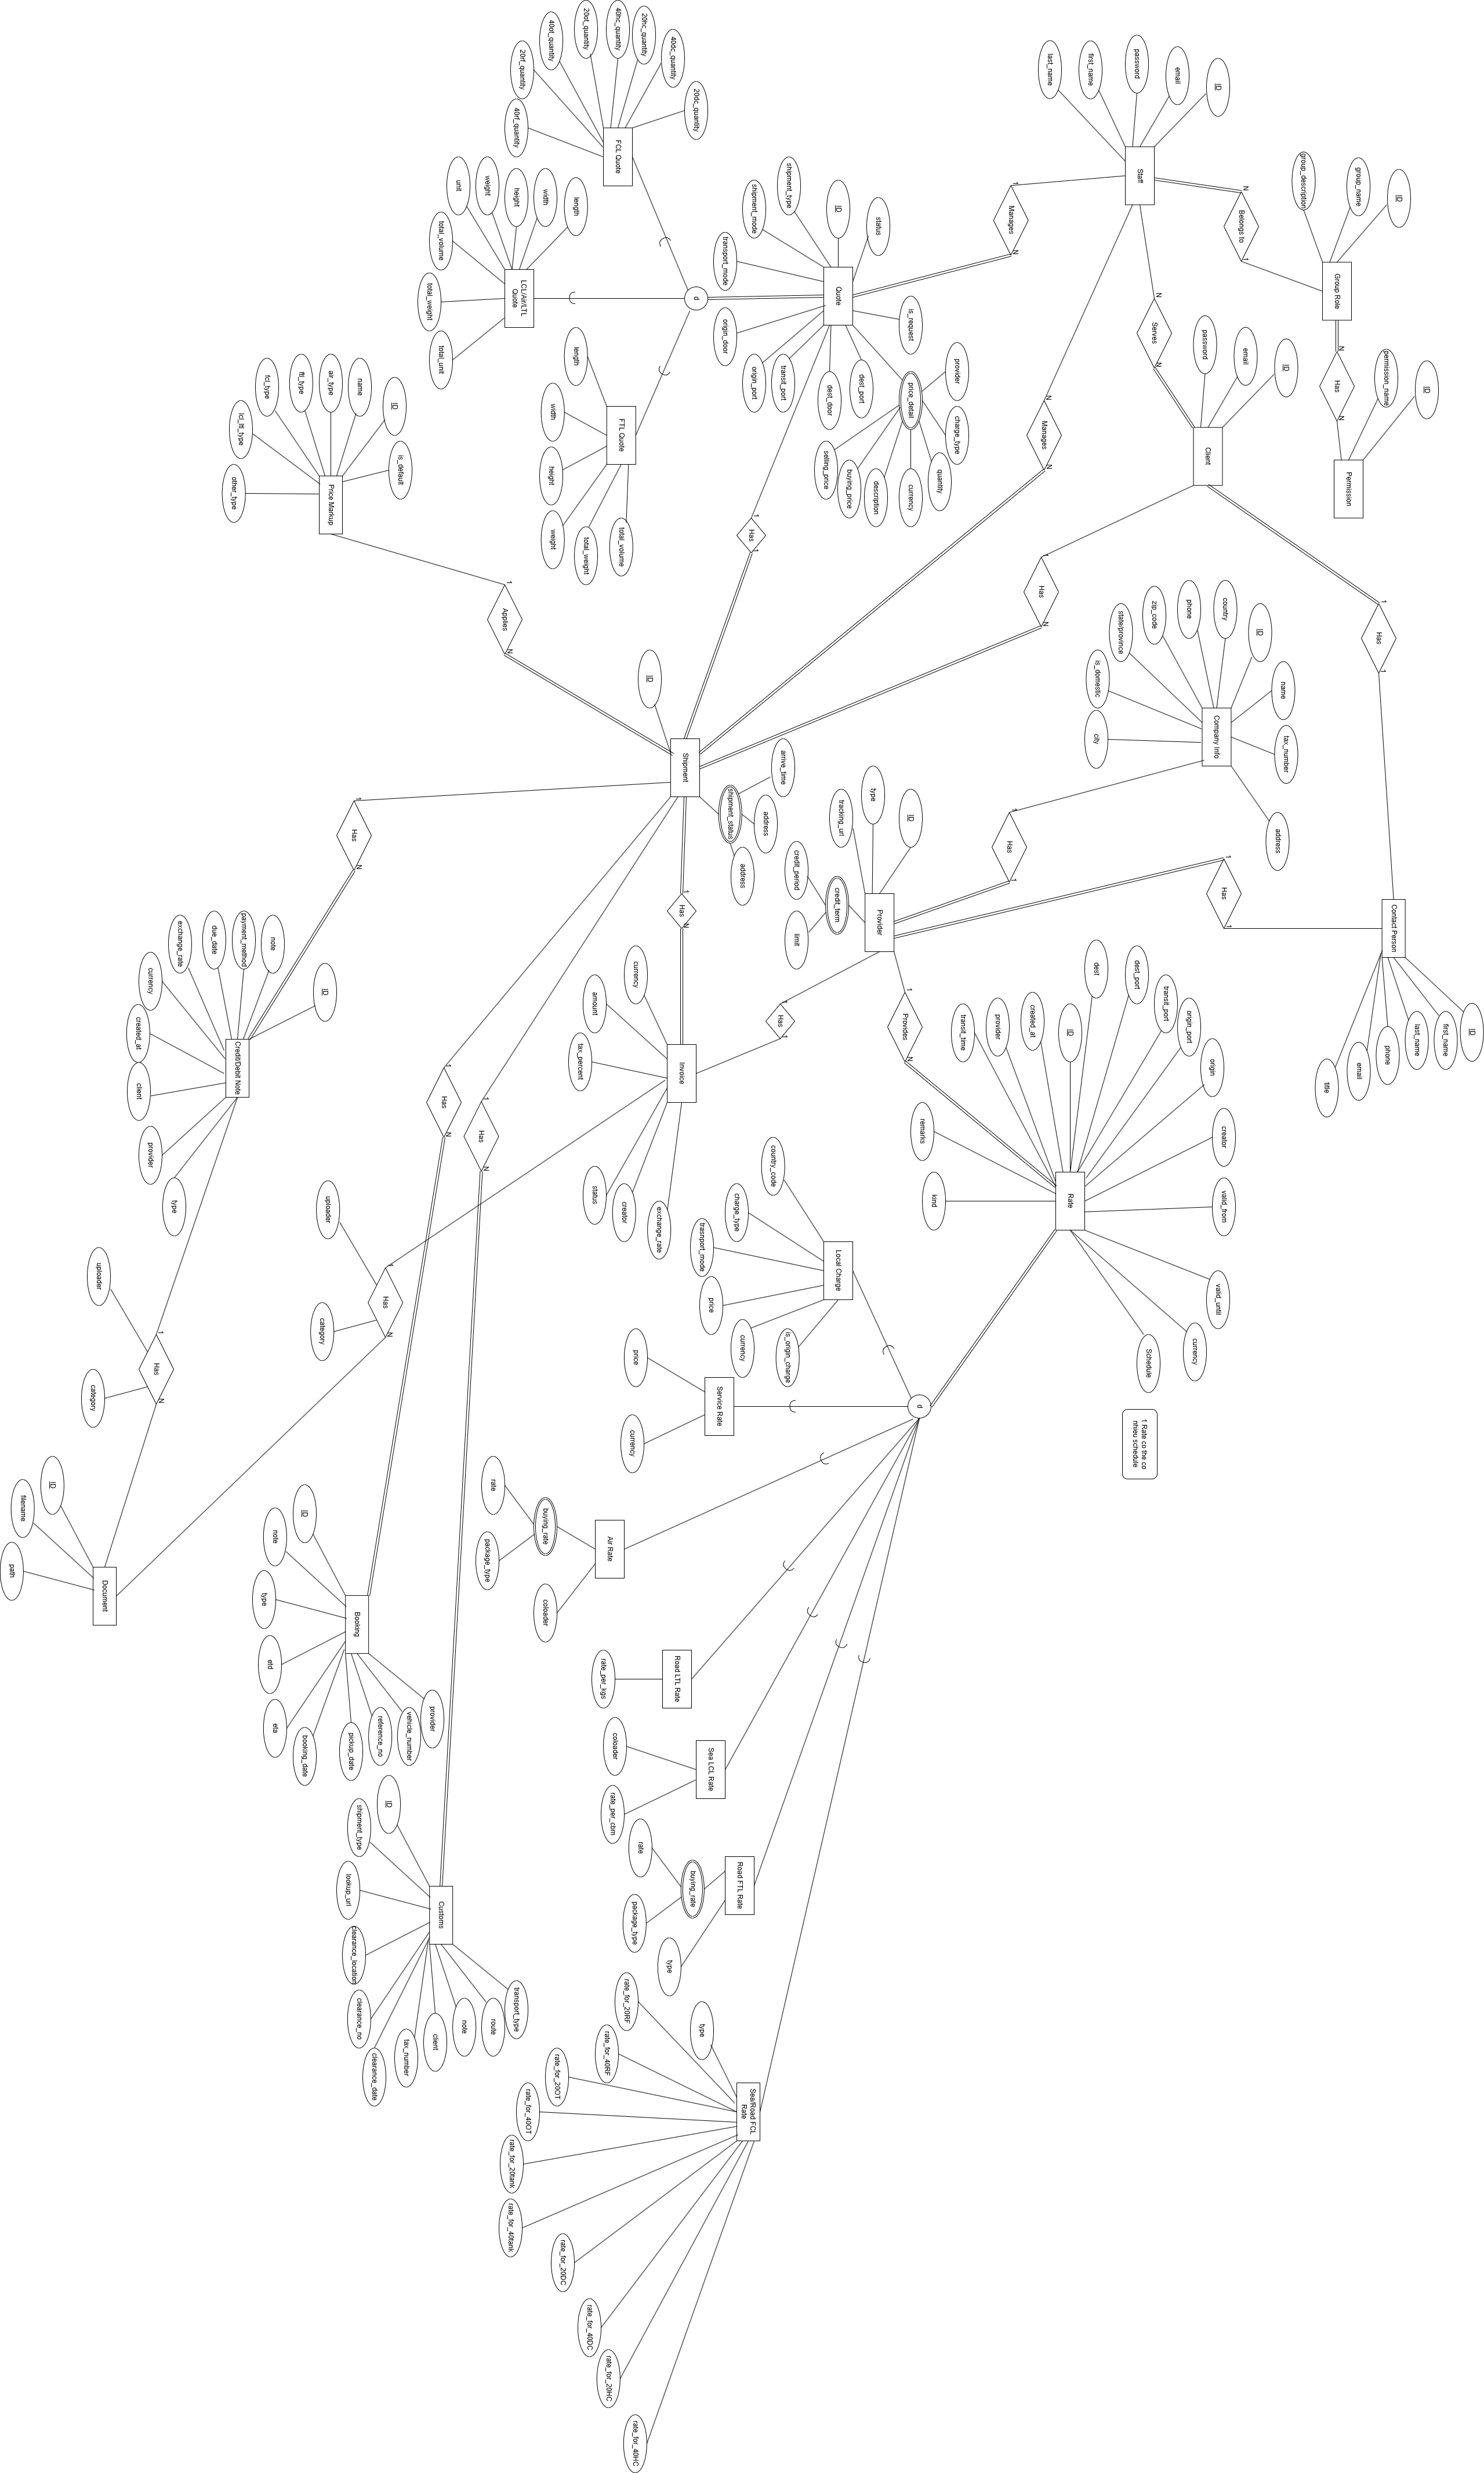
\includegraphics[width=\textwidth, height=\textheight, keepaspectratio]{graphics/DB/freight-flex-ERD.drawio.png}
    \caption{EERD}
    \label{fig:EERD}
\end{figure}

\begin{figure}[H]
    \centering
    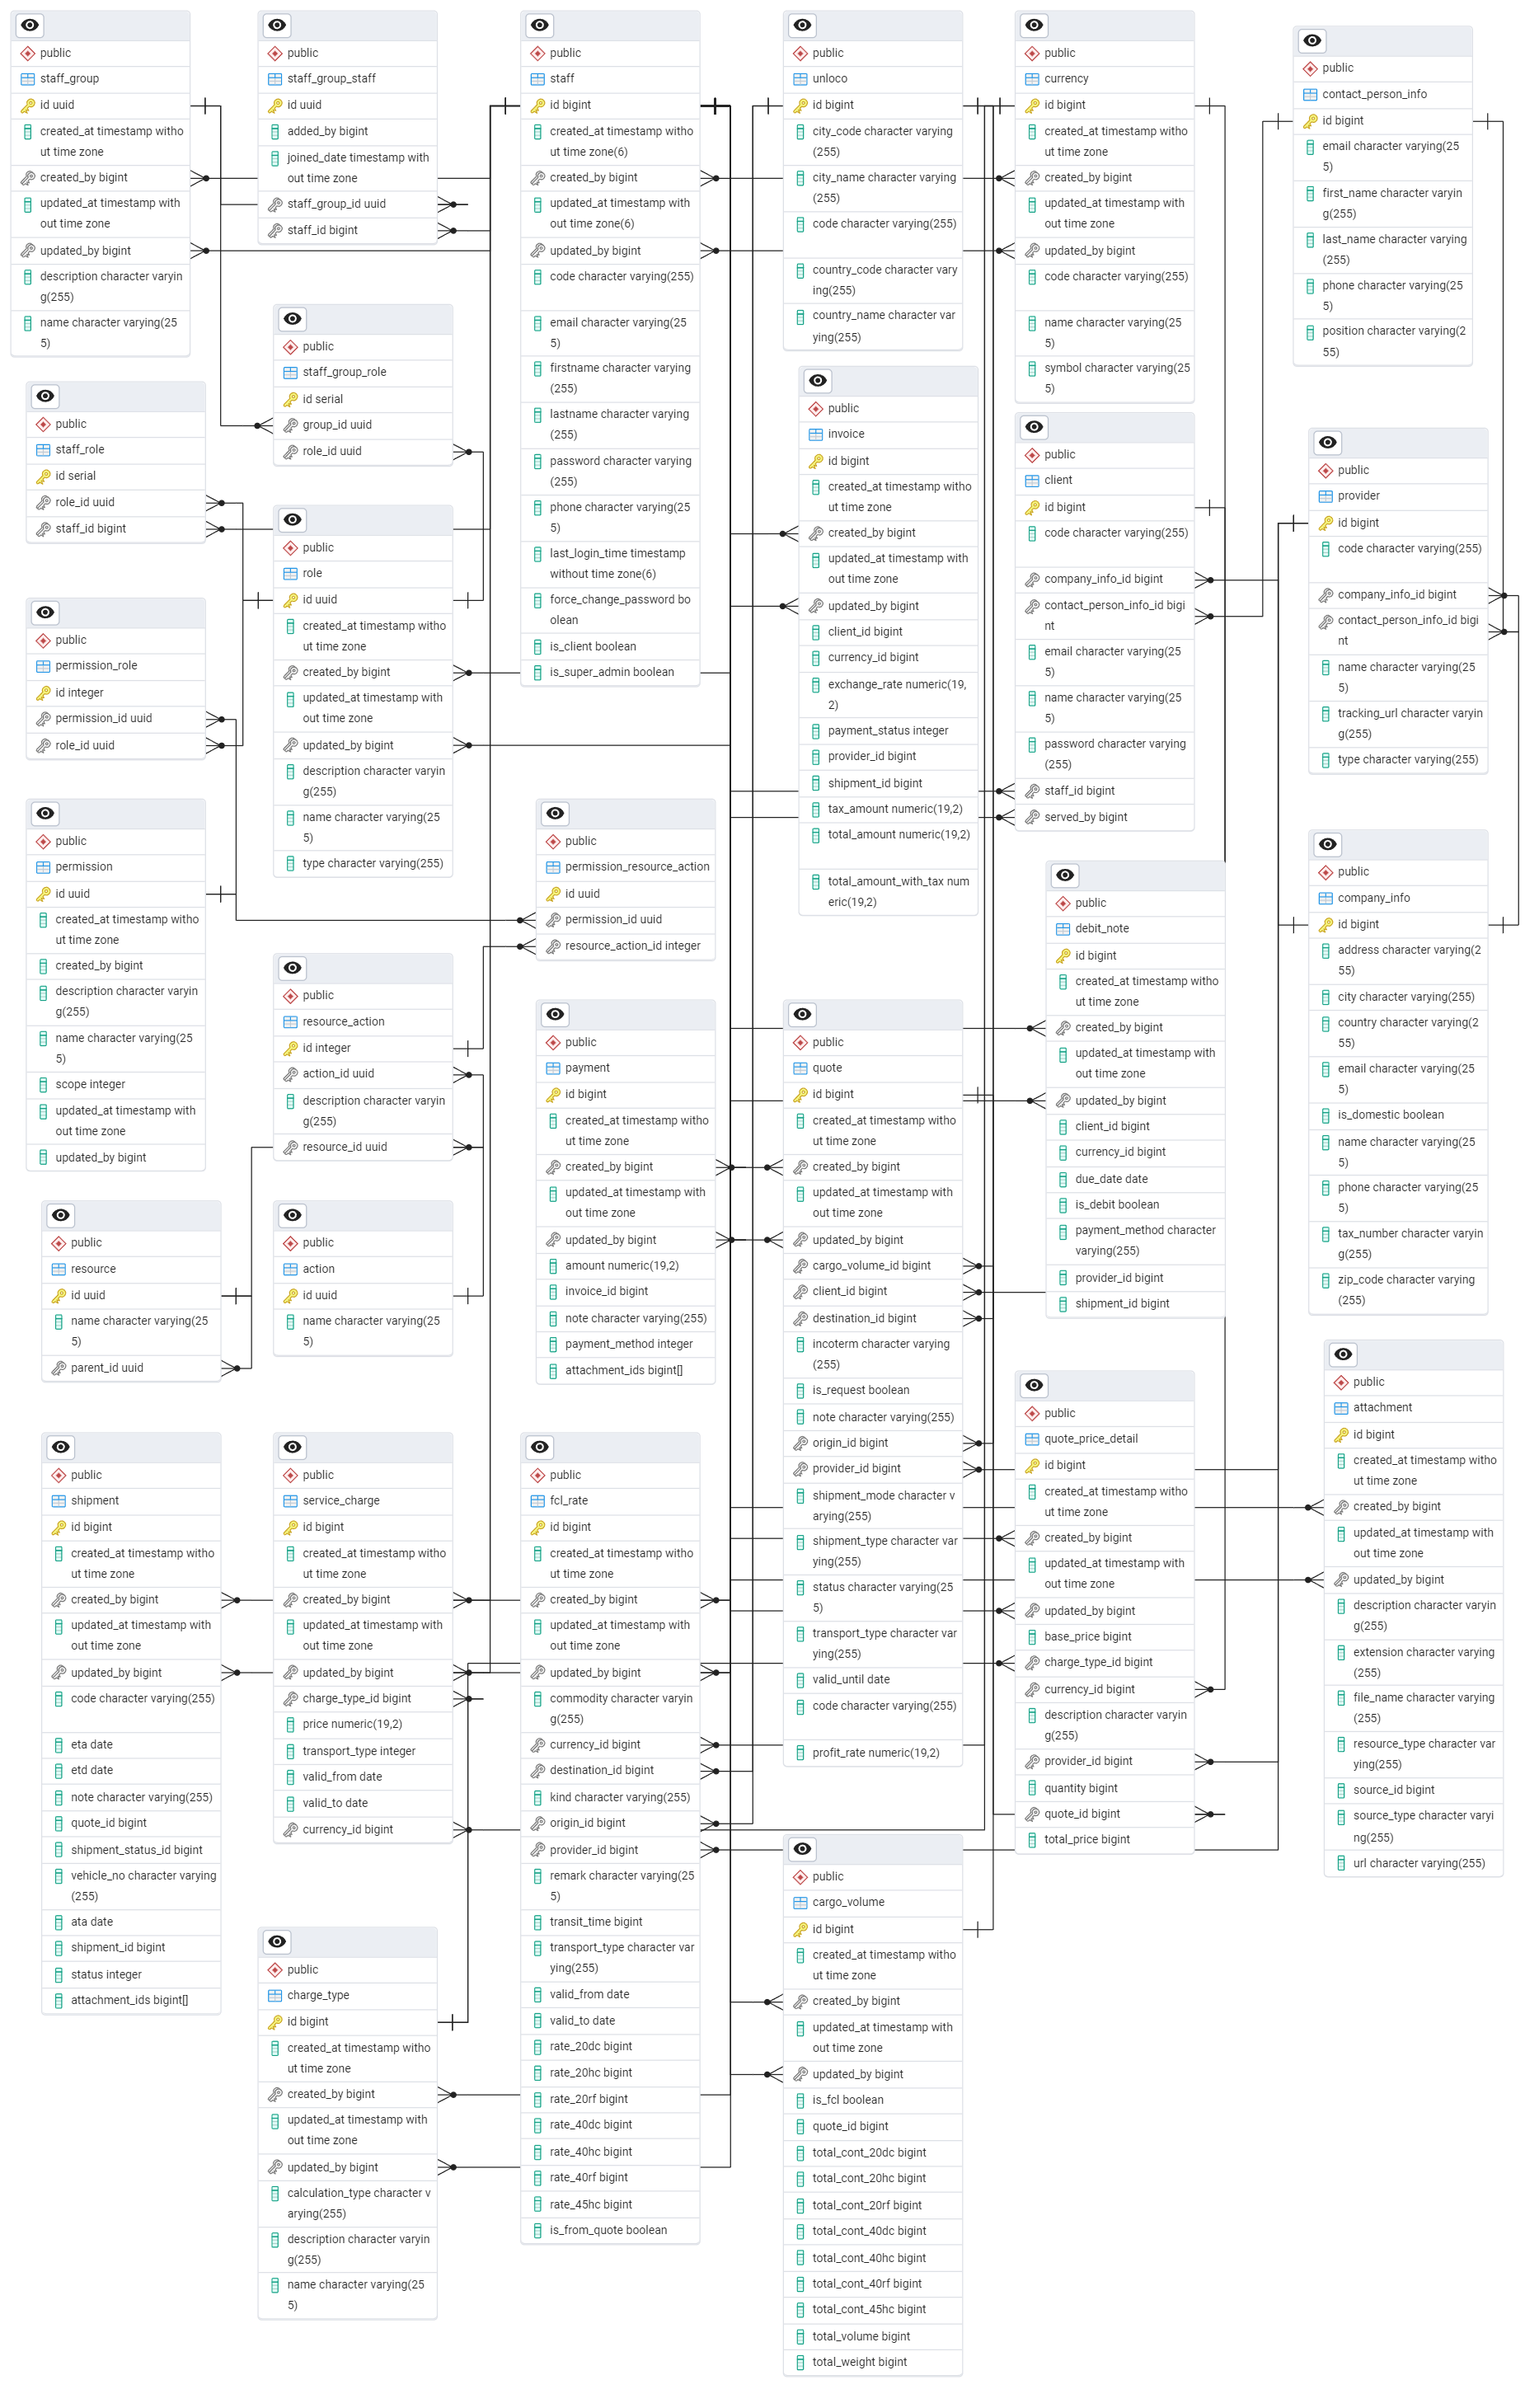
\includegraphics[width=\textwidth, height=\textheight, keepaspectratio]{graphics/DB/entity-mapping.png}
    \caption{Enitty Mapping}
    \label{fig:entity-mapping}
\end{figure}
% \subsection{Entity Detail}
% \subsubsection{staff}
% \begin{table}[H]
%     \centering
%     \begin{tabular}{|p{3cm}|p{2cm}|p{\dimexpr\textwidth-6.8cm}|} % Adjust widths as needed
%         \hline
%         \rowcolor[HTML]{C0C0C0} 
%         \textbf{Attribute} & \textbf{Type} & \textbf{Description} \\ \hline
%         \underline{id} & Integer & Primary key \\ \hline
%         email & String & Email for login \\ \hline
%         password & String & Password for login \\ \hline
%         firstname & String & First name \\ \hline
%         lastname & String & Last name \\ \hline
%         phone & String & Phone number \\ \hline
%         last\_login\_time & Timestamp & Last login time \\ \hline
%         created\_at & Timestamp & The time when the Staff is created \\ \hline
%         updated\_at & Timestamp & The time when the Staff is updated \\ \hline
%         created\_by & Integer & Foreign key to Staff \\ \hline
%         updated\_by & Integer & Foreign key to Staff \\ \hline
%     \end{tabular}
%     \caption{Table of Staff}
%     \label{tab:staff-table}
% \end{table}
% \subsubsection{staff\_group}
% \begin{table}[H]
%     \centering
%     \begin{tabular}{|p{3cm}|p{2cm}|p{\dimexpr\textwidth-6.8cm}|} % Adjust widths as needed
%         \hline
%         \rowcolor[HTML]{C0C0C0} 
%         \textbf{Attribute} & \textbf{Type} & \textbf{Description} \\ \hline
%         \underline{id} & UUID & Primary key \\ \hline
%         name & String & Group name \\ \hline
%         description & String & Group description \\ \hline
%         created\_at & Timestamp & The time when the Group is created \\ \hline
%         updated\_at & Timestamp & The time when the Group is updated \\ \hline
%         created\_by & Integer & Foreign key to Staff \\ \hline
%         updated\_by & Integer & Foreign key to Staff \\ \hline
%     \end{tabular}
%     \caption{Table of Staff Group}
%     \label{tab:group-table}
% \end{table}
% \subsubsection{staff\_group\_role}
% \begin{table}[H]
%     \centering
%     \begin{tabular}{|p{3cm}|p{2cm}|p{\dimexpr\textwidth-6.8cm}|} % Adjust widths as needed
%         \hline
%         \rowcolor[HTML]{C0C0C0} 
%         \textbf{Attribute} & \textbf{Type} & \textbf{Description} \\ \hline
%         \underline{id} & Integer & Primary key \\ \hline
%         group\_id & UUID & Foreign key to Group\\ \hline
%         role\_id & Integer & Foreign key to Staff\\ \hline
%     \end{tabular}
%     \caption{Table of Staff Group Role}
%     \label{tab:group-table}
% \end{table}
% \subsubsection{staff\_group\_staff} 
% \begin{table}[H]
%     \centering
%     \begin{tabular}{|p{3cm}|p{2cm}|p{\dimexpr\textwidth-6.8cm}|} % Adjust widths as needed
%         \hline
%         \rowcolor[HTML]{C0C0C0} 
%         \textbf{Attribute} & \textbf{Type} & \textbf{Description} \\ \hline
%         \underline{id} & UUID & Primary key \\ \hline
%         staff\_group\_id & UUID & Foreign key to Staff Group\\ \hline
%         staff\_id & Integer & Foreign key to Staff\\ \hline
%         joined\_date & Timestamp & The time when the Staff joined the group \\ \hline
%         added\_by & Integer & Foreign key to Staff \\ \hline
%     \end{tabular}
%     \caption{Table of Staff Group Role}
%     \label{tab:group-table}
% \end{table}
% \subsubsection{Permission}
% \begin{table}[H]
%     \centering
%     \begin{tabular}{|p{3cm}|p{2cm}|p{\dimexpr\textwidth-6.8cm}|} % Adjust widths as needed
%         \hline
%         \rowcolor[HTML]{C0C0C0} 
%         \textbf{Attribute} & \textbf{Type} & \textbf{Description} \\ \hline
%         \underline{id} & Integer & Primary key \\ \hline
%         permission\_name & String & Permission name \\ \hline
%     \end{tabular}
%     \caption{Table of Permission}
%     \label{tab:permission-table}
% \end{table}
% \subsubsection{Group Permission}
% \begin{table}[H]
%     \centering
%     \begin{tabular}{|p{3cm}|p{2cm}|p{\dimexpr\textwidth-6.8cm}|} % Adjust widths as needed
%         \hline
%         \rowcolor[HTML]{C0C0C0} 
%         \textbf{Attribute} & \textbf{Type} & \textbf{Description} \\ \hline
%         \underline{group\_id} & Integer & Foreign key to Group\\ \hline
%         \underline{permission\_id} & Integer & Foreign key to Permission\\ \hline
%     \end{tabular}
%     \caption{Table of Group Permission}
%     \label{tab:group-permission-table}
% \end{table}

% \subsubsection{Staff serves Client}
% \begin{table}[H]
%     \centering
%     \begin{tabular}{|p{3cm}|p{2cm}|p{\dimexpr\textwidth-6.8cm}|} % Adjust widths as needed
%         \hline
%         \rowcolor[HTML]{C0C0C0} 
%         \textbf{Attribute} & \textbf{Type} & \textbf{Description} \\ \hline
%         \underline{staff\_id} & Integer & Foreign key to Staff\\ \hline
%         \underline{client\_id} & Integer & Foreign key to Client\\ \hline
%     \end{tabular}
%     \caption{Table of Staff serves Client}
%     \label{tab:Staff-serves-client-table}
% \end{table}

% \subsubsection{Client}
% \begin{table}[H]
%     \centering
%     \begin{tabular}{|p{3cm}|p{2cm}|p{\dimexpr\textwidth-6.8cm}|} % Adjust widths as needed
%         \hline
%         \rowcolor[HTML]{C0C0C0} 
%         \textbf{Attribute} & \textbf{Type} & \textbf{Description} \\ \hline
%         \underline{id} & Integer & Primary key \\ \hline
%         email & String & Email for login \\ \hline
%         password & String & Password for login \\ \hline
%         first\_name & String & First name \\ \hline
%         last\_name & String & Last name \\ \hline
%         avatar\_url & String & Url to avatar \\ \hline
%         companyinfo\_id & Integer & Foreign key to Company info \\ \hline
%         contact\_person\_id & Integer & Foreign key to Contact Person \\ \hline
%         price\_markup\_id & Integer & Foreign key to Price Markup \\ \hline
%         credit\_term\_id & Integer & Foreign key to Credit Term \\ \hline
%     \end{tabular}
%     \caption{Table of Client}
%     \label{tab:client-table}
% \end{table}

% \subsubsection{Company Info}
% \begin{table}[H]
%     \centering
%     \begin{tabular}{|p{3cm}|p{2cm}|p{\dimexpr\textwidth-6.8cm}|} % Adjust widths as needed
%         \hline
%         \rowcolor[HTML]{C0C0C0} 
%         \textbf{Attribute} & \textbf{Type} & \textbf{Description} \\ \hline
%         \underline{id} & Integer & Primary key \\ \hline
%         name & String & Company name \\ \hline
%         address & String & Company address \\ \hline
%         email & String & Company email \\ \hline
%         zip\_code & String & Company zip\-code \\ \hline
%         phone\_number & String & Company phone number \\ \hline
%         country & String & Company country \\ \hline
%         website & String & Company website \\ \hline
%         tax\_number & String & Company tax number \\ \hline
%         is\_domestic & Boolean & Is domestic \\ \hline
%     \end{tabular}
%     \caption{Table of Company Info}
%     \label{tab:company-info-table}
% \end{table}

% \subsubsection{Contact Person}
% \begin{table}[H]
%     \centering
%     \begin{tabular}{|p{3cm}|p{2cm}|p{\dimexpr\textwidth-6.8cm}|} % Adjust widths as needed
%         \hline
%         \rowcolor[HTML]{C0C0C0} 
%         \textbf{Attribute} & \textbf{Type} & \textbf{Description} \\ \hline
%         \underline{id} & Integer & Primary key \\ \hline
%         firs\_name & String & Contact person first name \\ \hline
%         last\_name & String & Contact person last name \\ \hline
%         email & String & Contact person email \\ \hline
%         phone\_number & String & Contact person phone number \\ \hline
%         title & String & Contact person title \\ \hline
%     \end{tabular}
%     \caption{Table of Contact Person}
%     \label{tab:contact-person-table}
% \end{table}

% \subsubsection{Price Markup}
% \begin{table}[H]
%     \centering
%     \begin{tabular}{|p{3cm}|p{2cm}|p{\dimexpr\textwidth-6.8cm}|} % Adjust widths as needed
%         \hline
%         \rowcolor[HTML]{C0C0C0} 
%         \textbf{Attribute} & \textbf{Type} & \textbf{Description} \\ \hline
%         \underline{id} & Integer & Primary key \\ \hline
%         name & String & Price markup name \\ \hline
%         fcl\_type & String & Price markup of FCL shipment \\ \hline
%         ftl\_type & String & Price markup of FTL shipment \\ \hline
%         lcl\_ltl\_type & String & Price markup of LCL or LTL shipment \\ \hline
%         air\_type & String & Price markup of AIR shipment \\ \hline
%         is\_default & Boolean & Is default \\ \hline
%     \end{tabular}
%     \caption{Table of Price Markup}
%     \label{tab:price-markup-table}
% \end{table}

% \subsubsection{Credit Term}
% \begin{table}[H]
%     \centering
%     \begin{tabular}{|p{3cm}|p{2cm}|p{\dimexpr\textwidth-6.8cm}|} % Adjust widths as needed
%         \hline
%         \rowcolor[HTML]{C0C0C0} 
%         \textbf{Attribute} & \textbf{Type} & \textbf{Description} \\ \hline
%         \underline{id} & Integer & Primary key \\ \hline
%         credit\_period & Integer & The number of days allowed for credit starting from the shipment's departure date. \\ \hline
%         credit\_period & Integer & The amount of money allowed for credit starting from the shipment's departure date. \\ \hline
%     \end{tabular}
%     \caption{Table of Credit term}
%     \label{tab:credit-term-table}
% \end{table}

% \subsubsection{Staff manages Shipment}
% \begin{table}[H]
%     \centering
%     \begin{tabular}{|p{3cm}|p{2cm}|p{\dimexpr\textwidth-6.8cm}|} % Adjust widths as needed
%         \hline
%         \rowcolor[HTML]{C0C0C0} 
%         \textbf{Attribute} & \textbf{Type} & \textbf{Description} \\ \hline
%         staff\_id & Integer & Foreign key to Staff\\ \hline
%         shipment\_id & Integer & Foreign key to Shipment\\ \hline
%     \end{tabular}
%     \caption{Table of Staff manages Shipment}
%     \label{tab:staff-manages-shipment}
% \end{table}

% \subsubsection{Shipment}
% \begin{table}[H]
%     \centering
%     \begin{tabular}{|p{3cm}|p{2cm}|p{\dimexpr\textwidth-6.8cm}|} % Adjust widths as needed
%         \hline
%         \rowcolor[HTML]{C0C0C0} 
%         \textbf{Attribute} & \textbf{Type} & \textbf{Description} \\ \hline
%         \underline{id} & Integer & Primary key \\ \hline
%         quote\_id & Integer & Foreign key to Quote\\ \hline
%         price\_markup\_id & Integer & Foreign key to Price Markup\\ \hline
%     \end{tabular}
%     \caption{Table of Shipment}
%     \label{tab:shipment-table}
% \end{table}

% \subsubsection{Invoice}
% \begin{table}[H]
%     \centering
%     \begin{tabular}{|p{3cm}|p{2cm}|p{\dimexpr\textwidth-6.8cm}|} % Adjust widths as needed
%         \hline
%         \rowcolor[HTML]{C0C0C0} 
%         \textbf{Attribute} & \textbf{Type} & \textbf{Description} \\ \hline
%         \underline{id} & Integer & Primary key \\ \hline
%         shipment\_id & Integer & Foreign key to Shipment\\ \hline
%         client\_id & Integer & Foreign key to Client\\ \hline
%         provider\_id & Integer & Foreign key to Provider\\ \hline
%         currency & String & Currency unit\\ \hline
%         amount & Float & Total amount\\ \hline
%         tax\_percent & Int & Tax percent \\ \hline
%         status & String & Invoice status \\ \hline
%         created\_at & Timestamp & The time when the Invoice is created \\ \hline
%         creator & Integer & Foreign key to Staff \\ \hline
%         exchange\_rate & Float & Money exchange rate \\ \hline
%     \end{tabular}
%     \caption{Table of Invoice}
%     \label{tab:invoice-table}
% \end{table}

% \subsubsection{Port}
% \begin{table}[H]
%     \centering
%     \begin{tabular}{|p{3cm}|p{2cm}|p{\dimexpr\textwidth-6.8cm}|} % Adjust widths as needed
%         \hline
%         \rowcolor[HTML]{C0C0C0} 
%         \textbf{Attribute} & \textbf{Type} & \textbf{Description} \\ \hline
%         \underline{id} & Integer & Primary key \\ \hline
%         port\_name & String & Port name\\ \hline
%         is\_airport & Boolean & Is airport or ocean\\ \hline
%     \end{tabular}
%     \caption{Table of Port}
%     \label{tab:port-table}
% \end{table}

% \subsubsection{Provider}
% \begin{table}[H]
%     \centering
%     \begin{tabular}{|p{3cm}|p{2cm}|p{\dimexpr\textwidth-6.8cm}|} % Adjust widths as needed
%         \hline
%         \rowcolor[HTML]{C0C0C0} 
%         \textbf{Attribute} & \textbf{Type} & \textbf{Description} \\ \hline
%         \underline{id} & Integer & Primary key \\ \hline
%         name & String & Provider name \\ \hline
%         companyinfo\_id & Integer & Foreign key to Company info \\ \hline
%         contact\_person\_id & Integer & Foreign key to Contact Person \\ \hline
%         credit\_term\_id & Integer & Foreign key to Credit Term \\ \hline
%     \end{tabular}
%     \caption{Table of Provider}
%     \label{tab:provider-table}
% \end{table}

% \subsubsection{Sea FCL Rate}
% \begin{table}[H]
%     \centering
%     \begin{tabular}{|p{3cm}|p{2cm}|p{\dimexpr\textwidth-6.8cm}|} % Adjust widths as needed
%         \hline
%         \rowcolor[HTML]{C0C0C0} 
%         \textbf{Attribute} & \textbf{Type} & \textbf{Description} \\ \hline
%         \underline{id} & Integer & Primary key \\ \hline
%         provider\_id & Integer & Foreign key to Provider\\ \hline
%         origin\_port\_id & Integer & Foreign key to Origin port\\ \hline
%         transit\_port\_id & Integer & Foreign key to Transit port\\ \hline
%         dest\_port\_id & Integer & Foreign key to Destination port\\ \hline
%         currency\_id & Integer & Foreign key to Currency\\ \hline
%         transit\_time & Integer & Amount of days to transit\\ \hline
%         remarks & String & Remarks\\ \hline
%         schedule & Date[] & A list of the days of the week when the ship can depart\\ \hline
%         rate\_for\_20dc & Integer & Rate for container type 20dc\\ \hline
%         rate\_for\_40dc & Integer & Rate for container type 40dc\\ \hline
%         rate\_for\_20hc & Integer & Rate for container type 20hc\\ \hline
%         rate\_for\_40hc & Integer & Rate for container type 40hc\\ \hline
%         rate\_for\_20ot & Integer & Rate for container type 20ot\\ \hline
%         rate\_for\_40ot & Integer & Rate for container type 40ot\\ \hline
%         rate\_for\_20rf & Integer & Rate for container type 20rf\\ \hline
%         rate\_for\_40rf & Integer & Rate for container type 40rf\\ \hline
%     \end{tabular}
%     \caption{Sea FCL Rate table}
%     \label{tab:sea-fcl-rate-table}
% \end{table}

% \subsubsection{Road FCL Rate}
% \begin{table}[H]
%     \centering
%     \begin{tabular}{|p{3cm}|p{2cm}|p{\dimexpr\textwidth-6.8cm}|} % Adjust widths as needed
%         \hline
%         \rowcolor[HTML]{C0C0C0} 
%         \textbf{Attribute} & \textbf{Type} & \textbf{Description} \\ \hline
%         \underline{id} & Integer & Primary key \\ \hline
%         provider\_id & Integer & Foreign key to Provider\\ \hline
%         currency\_id & Integer & Foreign key to Currency\\ \hline
%         origin\_door & String & Origin warehouse address\\ \hline
%         dest\_door & String & Destination warehouse address\\ \hline
%         transit\_time & Integer & Amount of days to transit\\ \hline
%         remarks & String & Remarks\\ \hline
%         schedule & Date[] & A list of the days of the week when the ship can depart\\ \hline
%         rate\_for\_20dc & Integer & Rate for container type 20dc\\ \hline
%         rate\_for\_40dc & Integer & Rate for container type 40dc\\ \hline
%         rate\_for\_20hc & Integer & Rate for container type 20hc\\ \hline
%         rate\_for\_40hc & Integer & Rate for container type 40hc\\ \hline
%         rate\_for\_20ot & Integer & Rate for container type 20ot\\ \hline
%         rate\_for\_40ot & Integer & Rate for container type 40ot\\ \hline
%         rate\_for\_20rf & Integer & Rate for container type 20rf\\ \hline
%         rate\_for\_40rf & Integer & Rate for container type 40rf\\ \hline
%     \end{tabular}
%     \caption{Road FCL Rate table}
%     \label{tab:road-fcl-rate-table}
% \end{table}

% \subsubsection{Sea LCL Rate}
% \begin{table}[H]
%     \centering
%     \begin{tabular}{|p{3cm}|p{2cm}|p{\dimexpr\textwidth-6.8cm}|} % Adjust widths as needed
%         \hline
%         \rowcolor[HTML]{C0C0C0} 
%         \textbf{Attribute} & \textbf{Type} & \textbf{Description} \\ \hline
%         \underline{id} & Integer & Primary key \\ \hline
%         provider\_id & Integer & Foreign key to Provider\\ \hline
%         origin\_port\_id & Integer & Foreign key to Origin port\\ \hline
%         transit\_port\_id & Integer & Foreign key to Transit port\\ \hline
%         dest\_port\_id & Integer & Foreign key to Destination port\\ \hline
%         currency\_id & Integer & Foreign key to Currency\\ \hline
%         transit\_time & Integer & Amount of days to transit\\ \hline
%         remarks & String & Remarks\\ \hline
%         schedule & Date[] & A list of the days of the week when the ship can depart\\ \hline
%         rate\_per\_cbm & Integer & Rate per cubic meter of goods\\ \hline
%     \end{tabular}
%     \caption{Sea LCL Rate table}
%     \label{tab:sea-lcl-rate-table}
% \end{table}

% \subsubsection{Road LCL Rate}
% \begin{table}[H]
%     \centering
%     \begin{tabular}{|p{3cm}|p{2cm}|p{\dimexpr\textwidth-6.8cm}|} % Adjust widths as needed
%         \hline
%         \rowcolor[HTML]{C0C0C0} 
%         \textbf{Attribute} & \textbf{Type} & \textbf{Description} \\ \hline
%         \underline{id} & Integer & Primary key \\ \hline
%         provider\_id & Integer & Foreign key to Provider\\ \hline
%         currency\_id & Integer & Foreign key to Currency\\ \hline
%         origin\_door & String & Origin warehouse address\\ \hline
%         dest\_door & String & Destination warehouse address\\ \hline
%         transit\_time & Integer & Amount of days to transit\\ \hline
%         remarks & String & Remarks\\ \hline
%         schedule & Date[] & A list of the days of the week when the ship can depart\\ \hline
%     \end{tabular}
%     \caption{Road LCL Rate table}
%     \label{tab:road-Lcl-rate-table}
% \end{table}

% \subsubsection{Quote}
% \begin{table}[H]
%     \centering
%     \begin{tabular}{|p{3cm}|p{2cm}|p{\dimexpr\textwidth-6.8cm}|} % Adjust widths as needed
%         \hline
%         \rowcolor[HTML]{C0C0C0} 
%         \textbf{Attribute} & \textbf{Type} & \textbf{Description} \\ \hline
%         \underline{id} & Integer & Primary key \\ \hline
%         status & Boolean & Status of the quote \\ \hline
%         shipment\_type & Integer & Type of the shipment \\ \hline
%         shipment\_mode & Integer & Mode of the shipment \\ \hline
%         transport\_mode & Integer & Mode of the transport \\ \hline
%         origin\_door & String & Address of the origin door \\ \hline
%         origin\_port & Integer & Id of the origin\_port \\ \hline
%         transit\_port & Integer & Id of transshipment port \\ \hline
%         dest\_door & String & Address of the destination port \\ \hline
%         dest\_port & Integer & Id of destination port \\ \hline
%         is\_request & Boolean & Is a quotations \\ \hline
%     \end{tabular}
%     \caption{Quote table}
%     \label{tab:quote-table}
% \end{table}

% \subsubsection{FCL Quote}
% \begin{table}[H]
%     \centering
%     \begin{tabular}{|p{3cm}|p{2cm}|p{\dimexpr\textwidth-6.8cm}|} % Adjust widths as needed
%         \hline
%         \rowcolor[HTML]{C0C0C0} 
%         \textbf{Attribute} & \textbf{Type} & \textbf{Description} \\ \hline
%         \underline{id} & Integer & Foreign key to staff \\ \hline
%         quote\_id & Integer & Foreign key to quote\\ \hline
%         20dc\_quantity & Integer & Number of container type 20dc\\ \hline
%         40dc\_quantity & Integer & Number of container type 40dc\\ \hline
%         20hc\_quantity & Integer & Number of container type 20hc\\ \hline
%         40hc\_quantity & Integer & Number of container type 40hc\\ \hline
%         20ot\_quantity & Integer & Number of container type 20ot\\ \hline
%         40ot\_quantity & Integer & Number of container type 40ot\\ \hline
%         20rf\_quantity & Integer & Number of container type 20rf\\ \hline
%         40rf\_quantity & Integer & Number of container type 40rf\\ \hline
%     \end{tabular}
%     \caption{FCL Quote table}
%     \label{tab:fcl-quote-table}
% \end{table}
% \subsubsection{LCL/Air/LTL Quote}
% \begin{table}[H]
%     \centering
%     \begin{tabular}{|p{3cm}|p{2cm}|p{\dimexpr\textwidth-6.8cm}|} % Adjust widths as needed
%         \hline
%         \rowcolor[HTML]{C0C0C0} 
%         \textbf{Attribute} & \textbf{Type} & \textbf{Description} \\ \hline
%         \underline{id} & Integer & Foreign key to staff \\ \hline
%         quote\_id & Integer & Foreign key to quote\\ \hline
%         length & Float & Length of a package\\ \hline
%         width & Float & width of a package\\ \hline
%         height & Float & height of a package\\ \hline
%         weight & Float & weight of a package\\ \hline
%         unit & String & unit of a package\\ \hline
%         total\_volumne & Float & Volumn of total package\\ \hline
%         total\_weight & Float & Weight of total package\\ \hline
%         total\_unit & String & Unit of total\\ \hline
%     \end{tabular}
%     \caption{LCL/Air/LTL Quote}
%     \label{tab:lcl-air-ltl-quote}
% \end{table}

% \subsubsection{FTL Quote}
% \begin{table}[H]
%     \centering
%     \begin{tabular}{|p{3cm}|p{2cm}|p{\dimexpr\textwidth-6.8cm}|} % Adjust widths as needed
%         \hline
%         \rowcolor[HTML]{C0C0C0} 
%         \textbf{Attribute} & \textbf{Type} & \textbf{Description} \\ \hline
%         \underline{id} & Integer & Foreign key to staff \\ \hline
%         quote\_id & Integer & Foreign key to quote\\ \hline
%         length & Float & Length of a package\\ \hline
%         width & Float & width of a package\\ \hline
%         height & Float & height of a package\\ \hline
%         weight & Float & weight of a package\\ \hline
%         total\_volumne & Float & Volumn of total package\\ \hline
%         total\_weight & Float & Weight of total package\\ \hline
%     \end{tabular}
%     \caption{FTL Quote}
%     \label{tab:ftl-quote}
% \end{table}
% \section{Entity Relationship Model}

\subsection{Entity Detail}

\subsubsection{Action}
\begin{table}[H]
    \centering
    \begin{tabular}{|p{3cm}|p{2cm}|p{\dimexpr\textwidth-6.8cm}|} % Adjust widths as needed
        \hline
        \rowcolor[HTML]{C0C0C0} 
        \textbf{Attribute} & \textbf{Type} & \textbf{Description} \\ \hline
        \underline{id} & UUID & Primary key \\ \hline
        name & String & Action name \\ \hline
    \end{tabular}
    \caption{Table of Action}
    \label{tab:action-table}
\end{table}

\subsubsection{Resource}
\begin{table}[H]
    \centering
    \begin{tabular}{|p{3cm}|p{2cm}|p{\dimexpr\textwidth-6.8cm}|} % Adjust widths as needed
        \hline
        \rowcolor[HTML]{C0C0C0} 
        \textbf{Attribute} & \textbf{Type} & \textbf{Description} \\ \hline
        \underline{id} & UUID & Primary key \\ \hline
        name & String & Resource name \\ \hline
        parent\_id & UUID & Foreign key to Resource \\ \hline
    \end{tabular}
    \caption{Table of Resource}
    \label{tab:resource-table}
\end{table}

\subsubsection{Resource Action}
\begin{table}[H]
    \centering
    \begin{tabular}{|p{3cm}|p{2cm}|p{\dimexpr\textwidth-6.8cm}|} % Adjust widths as needed
        \hline
        \rowcolor[HTML]{C0C0C0} 
        \textbf{Attribute} & \textbf{Type} & \textbf{Description} \\ \hline
        \underline{id} & Integer & Primary key \\ \hline
        resource\_id & UUID & Foreign key to Resource \\ \hline
        action\_id & UUID & Foreign key to Action \\ \hline
        description & String & Description of the resource action \\ \hline
    \end{tabular}
    \caption{Table of Resource Action}
    \label{tab:resource-action-table}
\end{table}

\subsubsection{Staff}
\begin{table}[H]
    \centering
    \begin{tabular}{|p{3cm}|p{2cm}|p{\dimexpr\textwidth-6.8cm}|} % Adjust widths as needed
        \hline
        \rowcolor[HTML]{C0C0C0} 
        \textbf{Attribute} & \textbf{Type} & \textbf{Description} \\ \hline
        \underline{id} & Integer & Primary key \\ \hline
        code & String & Staff code \\ \hline
        email & String & Email for login \\ \hline
        password & String & Password for login \\ \hline
        firstname & String & First name \\ \hline
        lastname & String & Last name \\ \hline
        phone & String & Phone number \\ \hline
        last\_login\_time & Timestamp & Last login time \\ \hline
        created\_at & Timestamp & The time when the Staff is created \\ \hline
        updated\_at & Timestamp & The time when the Staff is updated \\ \hline
        created\_by & Integer & Foreign key to Staff \\ \hline
        updated\_by & Integer & Foreign key to Staff \\ \hline
    \end{tabular}
    \caption{Table of Staff}
    \label{tab:staff-table}
\end{table}

\subsubsection{Staff Group}
\begin{table}[H]
    \centering
    \begin{tabular}{|p{3cm}|p{2cm}|p{\dimexpr\textwidth-6.8cm}|} % Adjust widths as needed
        \hline
        \rowcolor[HTML]{C0C0C0} 
        \textbf{Attribute} & \textbf{Type} & \textbf{Description} \\ \hline
        \underline{id} & UUID & Primary key \\ \hline
        name & String & Group name \\ \hline
        description & String & Group description \\ \hline
        created\_at & Timestamp & The time when the Group is created \\ \hline
        updated\_at & Timestamp & The time when the Group is updated \\ \hline
        created\_by & Integer & Foreign key to Staff \\ \hline
        updated\_by & Integer & Foreign key to Staff \\ \hline
    \end{tabular}
    \caption{Table of Staff Group}
    \label{tab:staff-group-table}
\end{table}

\subsubsection{Staff Group Staff}
\begin{table}[H]
    \centering
    \begin{tabular}{|p{3cm}|p{2cm}|p{\dimexpr\textwidth-6.8cm}|} % Adjust widths as needed
        \hline
        \rowcolor[HTML]{C0C0C0} 
        \textbf{Attribute} & \textbf{Type} & \textbf{Description} \\ \hline
        \underline{id} & UUID & Primary key \\ \hline
        staff\_group\_id & UUID & Foreign key to Staff Group \\ \hline
        staff\_id & Integer & Foreign key to Staff \\ \hline
        joined\_date & Timestamp & The time when the Staff joined the group \\ \hline
        added\_by & Integer & Foreign key to Staff \\ \hline
    \end{tabular}
    \caption{Table of Staff Group Staff}
    \label{tab:staff-group-staff-table}
\end{table}

\subsubsection{Role}
\begin{table}[H]
    \centering
    \begin{tabular}{|p{3cm}|p{2cm}|p{\dimexpr\textwidth-6.8cm}|} % Adjust widths as needed
        \hline
        \rowcolor[HTML]{C0C0C0} 
        \textbf{Attribute} & \textbf{Type} & \textbf{Description} \\ \hline
        \underline{id} & UUID & Primary key \\ \hline
        name & String & Role name \\ \hline
        description & String & Role description \\ \hline
        type & String & Role type \\ \hline
        created\_at & Timestamp & The time when the Role is created \\ \hline
        updated\_at & Timestamp & The time when the Role is updated \\ \hline
        created\_by & Integer & Foreign key to Staff \\ \hline
        updated\_by & Integer & Foreign key to Staff \\ \hline
    \end{tabular}
    \caption{Table of Role}
    \label{tab:role-table}
\end{table}

\subsubsection{Staff Group Role}
\begin{table}[H]
    \centering
    \begin{tabular}{|p{3cm}|p{2cm}|p{\dimexpr\textwidth-6.8cm}|} % Adjust widths as needed
        \hline
        \rowcolor[HTML]{C0C0C0} 
        \textbf{Attribute} & \textbf{Type} & \textbf{Description} \\ \hline
        \underline{id} & Integer & Primary key \\ \hline
        group\_id & UUID & Foreign key to Staff Group \\ \hline
        role\_id & UUID & Foreign key to Role \\ \hline
    \end{tabular}
    \caption{Table of Staff Group Role}
    \label{tab:staff-group-role-table}
\end{table}

\subsubsection{Staff Role}
\begin{table}[H]
    \centering
    \begin{tabular}{|p{3cm}|p{2cm}|p{\dimexpr\textwidth-6.8cm}|} % Adjust widths as needed
        \hline
        \rowcolor[HTML]{C0C0C0} 
        \textbf{Attribute} & \textbf{Type} & \textbf{Description} \\ \hline
        \underline{id} & Integer & Primary key \\ \hline
        staff\_id & Integer & Foreign key to Staff \\ \hline
        role\_id & UUID & Foreign key to Role \\ \hline
    \end{tabular}
    \caption{Table of Staff Role}
    \label{tab:staff-role-table}
\end{table}

\subsubsection{Permission}
\begin{table}[H]
    \centering
    \begin{tabular}{|p{3cm}|p{2cm}|p{\dimexpr\textwidth-6.8cm}|} % Adjust widths as needed
        \hline
        \rowcolor[HTML]{C0C0C0} 
        \textbf{Attribute} & \textbf{Type} & \textbf{Description} \\ \hline
        \underline{id} & UUID & Primary key \\ \hline
        name & String & Permission name \\ \hline
        description & String & Permission description \\ \hline
        scope & Integer & Permission scope \\ \hline
        created\_at & Timestamp & The time when the Permission is created \\ \hline
        updated\_at & Timestamp & The time when the Permission is updated \\ \hline
        created\_by & Integer & Foreign key to Staff \\ \hline
        updated\_by & Integer & Foreign key to Staff \\ \hline
    \end{tabular}
    \caption{Table of Permission}
    \label{tab:permission-table}
\end{table}

\subsubsection{Permission Resource Action}
\begin{table}[H]
    \centering
    \begin{tabular}{|p{3cm}|p{2cm}|p{\dimexpr\textwidth-6.8cm}|} % Adjust widths as needed
        \hline
        \rowcolor[HTML]{C0C0C0} 
        \textbf{Attribute} & \textbf{Type} & \textbf{Description} \\ \hline
        \underline{id} & UUID & Primary key \\ \hline
        permission\_id & UUID & Foreign key to Permission \\ \hline
        resource\_action\_id & Integer & Foreign key to Resource Action \\ \hline
    \end{tabular}
    \caption{Table of Permission Resource Action}
    \label{tab:permission-resource-action-table}
\end{table}

\subsubsection{Permission Role}
\begin{table}[H]
    \centering
    \begin{tabular}{|p{3cm}|p{2cm}|p{\dimexpr\textwidth-6.8cm}|} % Adjust widths as needed
        \hline
        \rowcolor[HTML]{C0C0C0} 
        \textbf{Attribute} & \textbf{Type} & \textbf{Description} \\ \hline
        \underline{id} & Integer & Primary key \\ \hline
        permission\_id & UUID & Foreign key to Permission \\ \hline
        role\_id & UUID & Foreign key to Role \\ \hline
    \end{tabular}
    \caption{Table of Permission Role}
    \label{tab:permission-role-table}
\end{table}

\subsubsection{Company Info}
\begin{table}[H]
    \centering
    \begin{tabular}{|p{3cm}|p{2cm}|p{\dimexpr\textwidth-6.8cm}|} % Adjust widths as needed
        \hline
        \rowcolor[HTML]{C0C0C0} 
        \textbf{Attribute} & \textbf{Type} & \textbf{Description} \\ \hline
        \underline{id} & Integer & Primary key \\ \hline
        name & String & Company name \\ \hline
        address & String & Company address \\ \hline
        city & String & Company city \\ \hline
        country & String & Company country \\ \hline
        email & String & Company email \\ \hline
        zip\_code & String & Company zip\-code \\ \hline
        phone & String & Company phone number \\ \hline
        tax\_number & String & Company tax number \\ \hline
        is\_domestic & Boolean & Is domestic \\ \hline
    \end{tabular}
    \caption{Table of Company Info}
    \label{tab:company-info-table}
\end{table}

\subsubsection{Contact Person Info}
\begin{table}[H]
    \centering
    \begin{tabular}{|p{3cm}|p{2cm}|p{\dimexpr\textwidth-6.8cm}|} % Adjust widths as needed
        \hline
        \rowcolor[HTML]{C0C0C0} 
        \textbf{Attribute} & \textbf{Type} & \textbf{Description} \\ \hline
        \underline{id} & Integer & Primary key \\ \hline
        first\_name & String & Contact person first name \\ \hline
        last\_name & String & Contact person last name \\ \hline
        email & String & Contact person email \\ \hline
        phone & String & Contact person phone number \\ \hline
        position & String & Contact person position/title \\ \hline
    \end{tabular}
    \caption{Table of Contact Person Info}
    \label{tab:contact-person-info-table}
\end{table}

\subsubsection{Client}
\begin{table}[H]
    \centering
    \begin{tabular}{|p{4cm}|p{2cm}|p{\dimexpr\textwidth-7.8cm}|} % Adjust widths as needed
        \hline
        \rowcolor[HTML]{C0C0C0} 
        \textbf{Attribute} & \textbf{Type} & \textbf{Description} \\ \hline
        \underline{id} & Integer & Primary key \\ \hline
        code & String & Client code \\ \hline
        name & String & Client name \\ \hline
        email & String & Client email \\ \hline
        company\_info\_id & Integer & Foreign key to Company Info \\ \hline
        contact\_person\_info\_id & Integer & Foreign key to Contact Person Info \\ \hline
        staff\_id & Integer & Foreign key to Staff \\ \hline
    \end{tabular}
    \caption{Table of Client}
    \label{tab:client-table}
\end{table}

\subsubsection{Provider}
\begin{table}[H]
    \centering
    \begin{tabular}{|p{4cm}|p{2cm}|p{\dimexpr\textwidth-7.8cm}|} % Adjust widths as needed
        \hline
        \rowcolor[HTML]{C0C0C0} 
        \textbf{Attribute} & \textbf{Type} & \textbf{Description} \\ \hline
        \underline{id} & Integer & Primary key \\ \hline
        code & String & Provider code \\ \hline
        name & String & Provider name \\ \hline
        type & String & Provider type \\ \hline
        tracking\_url & String & URL for tracking shipments \\ \hline
        company\_info\_id & Integer & Foreign key to Company Info \\ \hline
        contact\_person\_info\_id & Integer & Foreign key to Contact Person Info \\ \hline
    \end{tabular}
    \caption{Table of Provider}
    \label{tab:provider-table}
\end{table}

\subsubsection{UnLoCo (United Nations Location Code)}
\begin{table}[H]
    \centering
    \begin{tabular}{|p{3cm}|p{2cm}|p{\dimexpr\textwidth-6.8cm}|} % Adjust widths as needed
        \hline
        \rowcolor[HTML]{C0C0C0} 
        \textbf{Attribute} & \textbf{Type} & \textbf{Description} \\ \hline
        \underline{id} & Integer & Primary key \\ \hline
        code & String & Location code \\ \hline
        country\_code & String & Country code \\ \hline
        country\_name & String & Country name \\ \hline
        city\_code & String & City code \\ \hline
        city\_name & String & City name \\ \hline
    \end{tabular}
    \caption{Table of UnLoCo}
    \label{tab:unloco-table}
\end{table}

\subsubsection{Currency}
\begin{table}[H]
    \centering
    \begin{tabular}{|p{3cm}|p{2cm}|p{\dimexpr\textwidth-6.8cm}|} % Adjust widths as needed
        \hline
        \rowcolor[HTML]{C0C0C0} 
        \textbf{Attribute} & \textbf{Type} & \textbf{Description} \\ \hline
        \underline{id} & Integer & Primary key \\ \hline
        code & String & Currency code \\ \hline
        name & String & Currency name \\ \hline
        symbol & String & Currency symbol \\ \hline
        created\_at & Timestamp & The time when the Currency is created \\ \hline
        updated\_at & Timestamp & The time when the Currency is updated \\ \hline
        created\_by & Integer & Foreign key to Staff \\ \hline
        updated\_by & Integer & Foreign key to Staff \\ \hline
    \end{tabular}
    \caption{Table of Currency}
    \label{tab:currency-table}
\end{table}

\subsubsection{Charge Type}
\begin{table}[H]
    \centering
    \begin{tabular}{|p{3cm}|p{2cm}|p{\dimexpr\textwidth-6.8cm}|} % Adjust widths as needed
        \hline
        \rowcolor[HTML]{C0C0C0} 
        \textbf{Attribute} & \textbf{Type} & \textbf{Description} \\ \hline
        \underline{id} & Integer & Primary key \\ \hline
        name & String & Charge type name \\ \hline
        description & String & Charge type description \\ \hline
        calculation\_type & String & Type of calculation for charges \\ \hline
        created\_at & Timestamp & The time when the Charge Type is created \\ \hline
        updated\_at & Timestamp & The time when the Charge Type is updated \\ \hline
        created\_by & Integer & Foreign key to Staff \\ \hline
        updated\_by & Integer & Foreign key to Staff \\ \hline
    \end{tabular}
    \caption{Table of Charge Type}
    \label{tab:charge-type-table}
\end{table}

\subsubsection{Service Charge}
\begin{table}[H]
    \centering
    \begin{tabular}{|p{3cm}|p{3cm}|p{\dimexpr\textwidth-7.8cm}|} % Adjust widths as needed
        \hline
        \rowcolor[HTML]{C0C0C0} 
        \textbf{Attribute} & \textbf{Type} & \textbf{Description} \\ \hline
        \underline{id} & Integer & Primary key \\ \hline
        charge\_type\_id & Integer & Foreign key to Charge Type \\ \hline
        price & Numeric(19, 2) & Price amount \\ \hline
        currency\_id & Integer & Foreign key to Currency \\ \hline
        transport\_type & Integer & Type of transport \\ \hline
        valid\_from & Date & Start date of validity \\ \hline
        valid\_to & Date & End date of validity \\ \hline
        created\_at & Timestamp & The time when the Service Charge is created \\ \hline
        updated\_at & Timestamp & The time when the Service Charge is updated \\ \hline
        created\_by & Integer & Foreign key to Staff \\ \hline
        updated\_by & Integer & Foreign key to Staff \\ \hline
    \end{tabular}
    \caption{Table of Service Charge}
    \label{tab:service-charge-table}
\end{table}

\subsubsection{FCL Rate}
\begin{table}[H]
    \centering
    \begin{tabular}{|p{3cm}|p{2cm}|p{\dimexpr\textwidth-6.8cm}|} % Adjust widths as needed
        \hline
        \rowcolor[HTML]{C0C0C0} 
        \textbf{Attribute} & \textbf{Type} & \textbf{Description} \\ \hline
        \underline{id} & Integer & Primary key \\ \hline
        provider\_id & Integer & Foreign key to Provider \\ \hline
        origin\_id & Integer & Foreign key to Origin UnLoCo \\ \hline
        destination\_id & Integer & Foreign key to Destination UnLoCo \\ \hline
        currency\_id & Integer & Foreign key to Currency \\ \hline
        kind & String & Kind of FCL rate \\ \hline
        transport\_type & String & Type of transport \\ \hline
        commodity & String & Type of goods \\ \hline
        transit\_time & Integer & Transit time in days \\ \hline
        remark & String & Additional remarks \\ \hline
        valid\_from & Date & Start date of validity \\ \hline
        valid\_to & Date & End date of validity \\ \hline
        is\_from\_quote & Boolean & Whether this rate is from a quote \\ \hline
        rate\_20dc & Integer & Rate for 20ft dry container \\ \hline
        rate\_40dc & Integer & Rate for 40ft dry container \\ \hline
        rate\_20hc & Integer & Rate for 20ft high cube container \\ \hline
        rate\_40hc & Integer & Rate for 40ft high cube container \\ \hline
        rate\_20rf & Integer & Rate for 20ft reefer container \\ \hline
        rate\_40rf & Integer & Rate for 40ft reefer container \\ \hline
        rate\_45hc & Integer & Rate for 45ft high cube container \\ \hline
        created\_at & Timestamp & The time when the FCL Rate is created \\ \hline
        updated\_at & Timestamp & The time when the FCL Rate is updated \\ \hline
        created\_by & Integer & Foreign key to Staff \\ \hline
        updated\_by & Integer & Foreign key to Staff \\ \hline
    \end{tabular}
    \caption{Table of FCL Rate}
    \label{tab:fcl-rate-table} 
\end{table}

\subsubsection{Quote}
\begin{table}[H]
    \centering
    \begin{tabular}{|p{3cm}|p{2cm}|p{\dimexpr\textwidth-6.8cm}|} % Adjust widths as needed
        \hline
        \rowcolor[HTML]{C0C0C0} 
        \textbf{Attribute} & \textbf{Type} & \textbf{Description} \\ \hline
        \underline{id} & Integer & Primary key \\ \hline
        client\_id & Integer & Foreign key to Client \\ \hline
        provider\_id & Integer & Foreign key to Provider \\ \hline
        origin\_id & Integer & Foreign key to Origin UnLoCo \\ \hline
        destination\_id & Integer & Foreign key to Destination UnLoCo \\ \hline
        cargo\_volume\_id & Integer & Foreign key to Cargo Volume \\ \hline
        shipment\_type & String & Type of shipment \\ \hline
        shipment\_mode & String & Mode of shipment \\ \hline
        transport\_type & String & Type of transport \\ \hline
        incoterm & String & International commercial terms \\ \hline
        is\_request & Boolean & Whether this is a quote request \\ \hline
        status & String & Status of the quote \\ \hline
        note & String & Additional notes \\ \hline
        valid\_until & Date & Quote validity end date \\ \hline
        created\_at & Timestamp & The time when the Quote is created \\ \hline
        updated\_at & Timestamp & The time when the Quote is updated \\ \hline
        created\_by & Integer & Foreign key to Staff \\ \hline
        updated\_by & Integer & Foreign key to Staff \\ \hline
    \end{tabular}
    \caption{Table of Quote}
    \label{tab:quote-table}
\end{table}

\subsubsection{Quote Price Detail}
\begin{table}[H]
    \centering
    \begin{tabular}{|p{3cm}|p{2cm}|p{\dimexpr\textwidth-6.8cm}|} % Adjust widths as needed
        \hline
        \rowcolor[HTML]{C0C0C0} 
        \textbf{Attribute} & \textbf{Type} & \textbf{Description} \\ \hline
        \underline{id} & Integer & Primary key \\ \hline
        quote\_id & Integer & Foreign key to Quote \\ \hline
        provider\_id & Integer & Foreign key to Provider \\ \hline
        charge\_type\_id & Integer & Foreign key to Charge Type \\ \hline
        description & String & Description of the price detail \\ \hline
        base\_price & Integer & Base price amount \\ \hline
        quantity & Integer & Quantity \\ \hline
        total\_price & Integer & Total price amount \\ \hline
        currency\_id & Integer & Foreign key to Currency \\ \hline
        created\_at & Timestamp & The time when the Quote Price Detail is created \\ \hline
        updated\_at & Timestamp & The time when the Quote Price Detail is updated \\ \hline
        created\_by & Integer & Foreign key to Staff \\ \hline
        updated\_by & Integer & Foreign key to Staff \\ \hline
    \end{tabular}
    \caption{Table of Quote Price Detail}
    \label{tab:quote-price-detail-table}
\end{table}

\subsubsection{Shipment}
\begin{table}[H]
    \centering
    \begin{tabular}{|p{3.5cm}|p{2cm}|p{\dimexpr\textwidth-7.3cm}|} % Adjust widths as needed
        \hline
        \rowcolor[HTML]{C0C0C0} 
        \textbf{Attribute} & \textbf{Type} & \textbf{Description} \\ \hline
        \underline{id} & Integer & Primary key \\ \hline
        code & String & Shipment code \\ \hline
        quote\_id & Integer & Foreign key to Quote \\ \hline
        etd & Date & Estimated time of departure \\ \hline
        eta & Date & Estimated time of arrival \\ \hline
        shipment\_status\_id & Integer & Foreign key to Shipment Status \\ \hline
        vehicle\_no & String & Vehicle number \\ \hline
        note & String & Additional notes \\ \hline
        attachment\_ids & Integer[] & Foreign key to Attachment \\ \hline
        created\_at & Timestamp & The time when the Shipment is created \\ \hline
        updated\_at & Timestamp & The time when the Shipment is updated \\ \hline
        created\_by & Integer & Foreign key to Staff \\ \hline
        updated\_by & Integer & Foreign key to Staff \\ \hline
    \end{tabular}
    \caption{Table of Shipment}
    \label{tab:shipment-table}
\end{table}

\subsubsection{Shipment Status}
\begin{table}[H]
    \centering
    \begin{tabular}{|p{3cm}|p{2cm}|p{\dimexpr\textwidth-6.8cm}|} % Adjust widths as needed
        \hline
        \rowcolor[HTML]{C0C0C0} 
        \textbf{Attribute} & \textbf{Type} & \textbf{Description} \\ \hline
        \underline{id} & Integer & Primary key \\ \hline
        shipment\_id & Integer & Foreign key to Shipment \\ \hline
        status & String & Shipment status \\ \hline
        eta & Date & Estimated time of arrival \\ \hline
        ata & Date & Actual time of arrival \\ \hline
        note & String & Additional notes \\ \hline
        created\_at & Timestamp & The time when the Shipment Status is created \\ \hline
        updated\_at & Timestamp & The time when the Shipment Status is updated \\ \hline
        created\_by & Integer & Foreign key to Staff \\ \hline
        updated\_by & Integer & Foreign key to Staff \\ \hline
    \end{tabular}
    \caption{Table of Shipment Status}
    \label{tab:shipment-status-table}
\end{table}

\subsubsection{Invoice}
\begin{table}[H]
    \centering
    \begin{tabular}{|p{4cm}|p{3cm}|p{\dimexpr\textwidth-8.8cm}|} % Adjust widths as needed
        \hline
        \rowcolor[HTML]{C0C0C0} 
        \textbf{Attribute} & \textbf{Type} & \textbf{Description} \\ \hline
        \underline{id} & Integer & Primary key \\ \hline
        shipment\_id & Integer & Foreign key to Shipment \\ \hline
        provider\_id & Integer & Foreign key to Provider \\ \hline
        client\_id & Integer & Foreign key to Client \\ \hline
        currency\_id & Integer & Foreign key to Currency \\ \hline
        total\_amount & Numeric(19, 2) & Total amount \\ \hline
        tax\_amount & Numeric(19, 2) & Tax amount \\ \hline
        total\_amount\_with\_tax & Numeric(19, 2) & Total amount with tax \\ \hline
        payment\_status & String & Payment status \\ \hline
        exchange\_rate & Numeric(19, 4) & Exchange rate \\ \hline
        created\_at & Timestamp & The time when the Invoice is created \\ \hline
        updated\_at & Timestamp & The time when the Invoice is updated \\ \hline
        created\_by & Integer & Foreign key to Staff \\ \hline
        updated\_by & Integer & Foreign key to Staff \\ \hline
    \end{tabular}
    \caption{Table of Invoice}
    \label{tab:invoice-table}
\end{table}

\subsubsection{Debit/Credit Note}
\begin{table}[H]
    \centering
    \begin{tabular}{|p{3cm}|p{2cm}|p{\dimexpr\textwidth-6.8cm}|} % Adjust widths as needed
        \hline
        \rowcolor[HTML]{C0C0C0} 
        \textbf{Attribute} & \textbf{Type} & \textbf{Description} \\ \hline
        \underline{id} & Integer & Primary key \\ \hline
        is\_debit & Boolean & Is debit note \\ \hline
        shipment\_id & Integer & Foreign key to Shipment \\ \hline
        provider\_id & Integer & Foreign key to Provider \\ \hline
        client\_id & Integer & Foreign key to Client \\ \hline
        currency\_id & Integer & Foreign key to Currency \\ \hline
        due\_date & Date & Due date \\ \hline
        payment\_method & String & Payment method \\ \hline
        created\_at & Timestamp & The time when the Debit/Credit Note is created \\ \hline
        updated\_at & Timestamp & The time when the Debit/Credit Note is updated \\ \hline
        created\_by & Integer & Foreign key to Staff \\ \hline
        updated\_by & Integer & Foreign key to Staff \\ \hline
    \end{tabular}
    \caption{Table of Debit/Credit Note}
    \label{tab:debit-credit-note-table}
\end{table}

\subsubsection{Payment}
\begin{table}[H]
    \centering
    \begin{tabular}{|p{3cm}|p{3cm}|p{\dimexpr\textwidth-7.8cm}|} % Adjust widths as needed
        \hline
        \rowcolor[HTML]{C0C0C0} 
        \textbf{Attribute} & \textbf{Type} & \textbf{Description} \\ \hline
        \underline{id} & Integer & Primary key \\ \hline
        invoice\_id & Integer & Foreign key to Invoice \\ \hline
        amount & Numeric(19, 2) & Payment amount \\ \hline
        payment\_method & String & Payment method \\ \hline
        note & String & Additional notes \\ \hline
        extra\_data & String & Extra data \\ \hline
        attachment\_ids & Integer[] & Foreign key to Attachment \\ \hline
        created\_at & Timestamp & The time when the Payment is created \\ \hline
        updated\_at & Timestamp & The time when the Payment is updated \\ \hline
        created\_by & Integer & Foreign key to Staff \\ \hline
        updated\_by & Integer & Foreign key to Staff \\ \hline
    \end{tabular}
    \caption{Table of Payment}
    \label{tab:payment-table}
\end{table}

\section{System Architecture}
\begin{figure}[H]
    \centering
    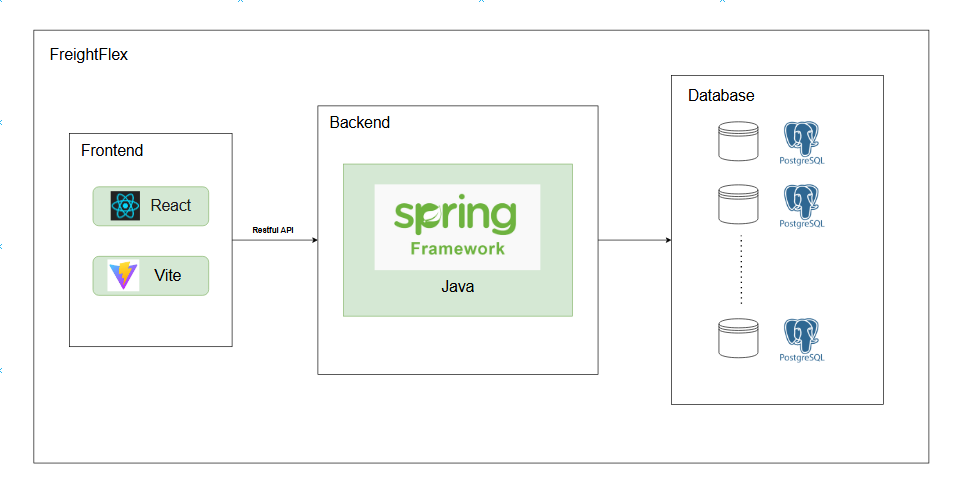
\includegraphics[width=15cm]{graphics/sys-design/system-architecture.png}
    \caption{FreightFlex Overall Architecture}
    \label{fig:FreightFlex Overall Architecture}
\end{figure}
After careful analysis of constraints such as human resources, development timelines, and maintainability requirements, the FreightFlex system adopts a client-server architectural pattern combined with an n-layer architecture for its backend. This decision balances system complexity with development efficiency while ensuring scalability and maintainability.

The frontend utilizes \texttt{React.js} with \texttt{Vite} for development, creating a robust client-side application that manages user interface rendering and state. This modern framework enables dynamic, responsive interfaces and high performance through virtual DOM implementation. \texttt{Vite} enhances the development experience with features like hot module replacement, reducing iteration cycles.

The backend is built with the \texttt{Spring Framework} in Java, structured in a layered architecture that promotes separation of concerns. This architecture comprises:
\begin{itemize}
    \item Presentation Layer (REST API controllers)
    \item Business Logic Layer (services)
    \item Data Access Layer (repositories)
    \item Domain Layer (entities and value objects)
\end{itemize}

The database employs a multi-tenant design using PostgreSQL's schema-based separation, which efficiently handles multiple freight forwarding companies (tenants) within a single database instance while maintaining strict data isolation. Key advantages include:

\begin{itemize}
    \item \textbf{Data Isolation:}
    \begin{itemize}
        \item Each tenant's data resides in its own schema.
        \item Cross-tenant data access is prevented through schema-level security.
    \end{itemize}
    
    \item \textbf{Resource Optimization:}
    \begin{itemize}
        \item Shared database instance reduces infrastructure costs.
        \item Efficient resource utilization via connection pooling.
    \end{itemize}
    
    \item \textbf{Tenant Management:}
    \begin{itemize}
        \item Dynamic tenant provisioning through automated schema creation.
        \item Flexible tenant-specific customizations.
    \end{itemize}
    
    \item \textbf{Performance Considerations:}
    \begin{itemize}
        \item Optimized query performance through schema-level indexing.
        \item Reduced database connection overhead.
    \end{itemize}
\end{itemize}

A centralized tenant management system supports this multi-tenant implementation, handling tenant registration, schema management, and data isolation enforcement.

This architectural approach maintains simplicity in client-server communication and provides several advantages for the freight forwarding system:
\begin{itemize}
    \item Clear separation of concerns for easier maintenance and enhancements.
    \item Scalable design for potential growth in functionality and user base.
    \item Secure multi-tenant implementation protecting sensitive data.
    \item Efficient resource utilization aligned with team capacity.
\end{itemize}

\section{Tools and Technologies Used}
\subsection{Frontend Technologies}
The frontend of the application is developed using the following technologies:
\begin{itemize}
    \item \textbf{React.js:} A popular JavaScript library for building user interfaces, enabling the creation of dynamic and responsive web applications.
    \item \textbf{Vite:} A modern build tool that enhances the development experience with features such as fast hot module replacement and optimized production builds.
    \item \textbf{Ant Design:} A comprehensive design system and UI component library that provides pre-built components for building aesthetically pleasing and user-friendly interfaces.
\end{itemize}

\subsection{Backend Technologies}
The backend is constructed using the following technologies:
\begin{itemize}
    \item \textbf{Java:} A robust, object-oriented programming language that serves as the foundation for backend development.
    \item \textbf{Spring Framework:} A powerful framework that simplifies Java application development, promoting good design practices through its modular architecture and dependency injection.
    \item \textbf{QueryDSL:} A framework that provides a type-safe way to construct SQL queries, enhancing the development process and maintaining code readability.
    \item \textbf{PostgreSQL:} An advanced, open-source relational database management system known for its reliability and performance, utilized for data storage and management.
\end{itemize}

\subsection{Development Tools}
The following tools are utilized to streamline the development process:
\begin{itemize}
    \item \textbf{Postman:} A collaboration platform for API development that provides tools for designing, testing, and documenting APIs.
    \item \textbf{Docker:} A containerization platform that enables the creation, deployment, and management of applications in isolated environments, ensuring consistency across different environments.
    \item \textbf{GitHub:} A web-based version control platform that facilitates collaboration among developers, providing tools for code management and version control.
    \item \textbf{Jira:} A project management tool that helps in tracking issues, managing tasks, and facilitating agile project management processes.
\end{itemize}

